\documentclass{llncs}
\usepackage{llncsdoc}
\usepackage[hidelinks]{hyperref}
\usepackage{listings}
\usepackage{graphicx}
\setcounter{secnumdepth}{4}
\setcounter{tocdepth}{4}

%
\begin{document}
\begin{flushleft}
 
 \thispagestyle{empty}
\centering\LARGE {\bf Software Vulnerability Management Techniques}




\vspace{2pt}


\centering
 Seminar: Selected Topics in Communication Management,
 Winter Term 2016/17



\centering
 Ehab Qadah\\
\rule{\textwidth}{1pt}



 

\end{flushleft}




\begin{abstract}
On a daily basis, new security flaws are discovered in software applications. This makes the software vulnerabilities analysis one of the top concerns for organizations. The automatic identification of vulnerable software inside the organization is fundamental to avoid cyber-attacks. In this paper, we discuss two techniques to automatically monitor software vulnerabilities using open standards and public vulnerability information repositories, and alternative method to identify a vulnerable software using information obtained from social media platforms. 
\end{abstract}

\section{Introduction}

\par Every year, new vulnerabilities are found in software products such as Internet Explorer, Flash 
 Player, and Java. According to Symantec \cite{symantec}, in 2015, the number of new vulnerabilities 
 reached 5,585, and 54 zero-day vulnerabilities were discovered. For cybercriminals 
 unpatched vulnerabilities represent an opportunity to carry out their attacks successfully. 
 Therefore, in order to prevent, for example, information theft, organizations require of 
 effective and efficient methods to automatically detect vulnerability in a software that is installed in 
 their networks. After detecting a software vulnerability, immediate actions (e.g., installing 
 patches, or preventing users from employing the vulnerable software) must be taken. 
 \par To automatically detect software vulnerabilities, organizations need a reliable source of 
 known vulnerabilities. Some solutions employ public repositories like the National 
 Vulnerability Database (NVD)\footnote{\url{https://nvd.nist.gov/}}. Then, organizations gather information on the software list that  
 installed in their networks to match that information with the vulnerabilities. 
 \par In this paper, we beginning with a brief explanation of the software vulnerability 
 management concept. Then, we describe standards used to unique identify software products 
 and vulnerabilities. Thereafter, we present two approaches for automated software vulnerability management. Next, we discuss key points of these approaches. Finally, we give the conclusion.
       
\section{Software Vulnerability Management}

In this section, we shortly describe the concept of Software Vulnerability Management. Before doing this we define what a software vulnerability is. In the field of information technology, a vulnerability is a defect or weakness in a system that leads to a security incident or unauthorized access to information or services by attackers \cite{vuln}.  

\par The Software Vulnerability Management concept can be defined as the process of identifying vulnerabilities in a software product that is installed inside an organization. The process first requires managing the inventory of the organization's IT assets; gathering the IT assets information and store it. Then,  periodically search for the related vulnerabilities. In case of the discovery of a vulnerability, certain actions should be performed such as alerting the system's administrator or installing the corresponding patches to avoid possible threats based on those vulnerabilities. Figure 1 shows the basic operations of the Software Vulnerability Management System.

\begin{figure}
 
  \centering
    \includegraphics[width=0.5\textwidth]{SVM.png}
     \caption{Basic operations of Software Vulnerability Management System}
\end{figure}

\section{Standards	Used	in	Software	Vulnerability	Management}
 
 In	this section, we describe three	components which are part of the Security	 Content	Automation	Protocol (SCAP)\footnote{\url{https://scap.nist.gov/}}. This protocol is a collection of open standards and enumerations for the	security  software flaws	 and configuration issues, the exchange of these	standards	offers	the	ability	to	automate	vulnerability	management \cite{scap_doc}.		
 SCAP is provided	and	maintained	by	the	National	Institute	of	Standards	and	Technology (NIST)\footnote{\url{https://www.nist.gov/}}. The SCAP	content	is	publicly accessible via  NVD, which is also managed	by NIST.
 
 
 \subsection{Common Vulnerabilities and Exposures (CVE®)} 
 CVE\footnote{\url{https://cve.mitre.org/index.html}} is a list of known security software venerabilities (available in XML format). To each vulnerability, a unique standard identifiers (e.g., CVE-2016-7892) is assigned. The CVE standard identifiers allow the data exchange between security solutions and vulnerability repositories (e.g., NVD, Japan Vulnerability Notes (JVN)\footnote{\url{https://jvn.jp/en/}} ). The CVE list is managed by The MITRE Corporation\footnote{\url{https://www.mitre.org/}}.

 The CVE list is not a vulnerability repository\footnote{The list of vulnerability databases list can be found at \url{https://cve.mitre.org/compatible/product_type.html\#Vulnerability Database}}, but a list of identifiers (i.e., CVE names) for  known vulnerabilities with basic information such as standard identifier and description. The CVE common identifiers of security vulnerabilities allow the linking between different vulnerability repositories. For example, NVD, JVN, and Symantec Security Response Web site \footnote{\url{https://www.symantec.com/security_response/landing/vulnerabilities.jsp}}. The linking between these databases allows to aggregate information about a vulnerability form all of them. 
 
 NVD provides an XML vulnerability feed that is built based on the CVE list. Based on the XML feed schema \footnote{\url{https://scap.nist.gov/schema/nvd/vulnerability_0.4.xsd}}, each vulnerability entry contains CVE id, summary, vulnerable software list, etc. Figure 2 shows an example CVE entry (CVE-2014-6348) with basic information obtained from NVD XML feed.
  \newpage
  \begin{figure}
    \centering
      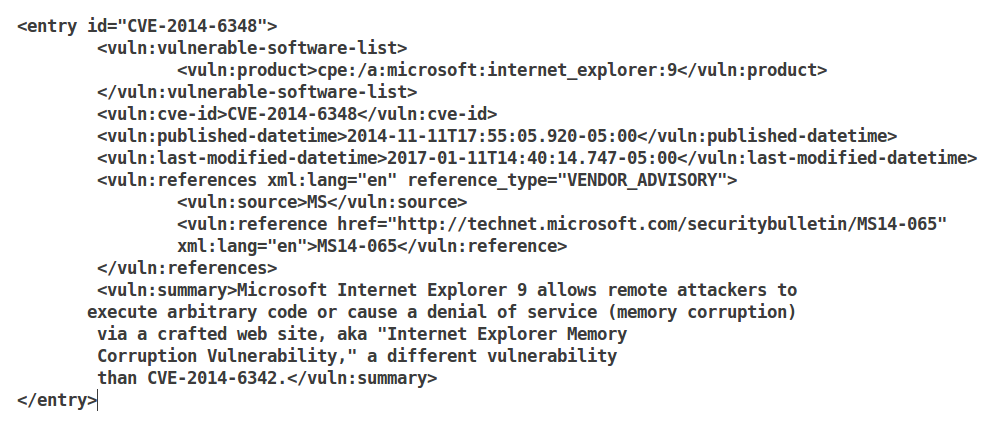
\includegraphics[width=\textwidth]{cve.png}
       \caption{Basic information of CVE-2014-6348 entry, some other information are omitted. }
  \end{figure}
 
 \subsection{Common Platform Enumeration (CPE™)}
 CPE\footnote{\url{https://cpe.mitre.org/specification/}} is the identifiers dictionary for the software products and applications,operating systems and hardware devices. The official CPE dictionary (current version is 2.3) \footnote{The Official CPE Dictionary available at \url{https://nvd.nist.gov/cpe.cfm}} provided in XML format by NVD and it is updated frequently.
 \par The CPE ID based upon the generic syntax for Uniform Resource Identifiers (URI), it follows the structure of \textbf{cpe:/ \{part\}:\{vendor\}:\{product\}:\{version\}:
 \{update\}:\{edition\}:\{lang\}} (e.g., cpe:/o:microsoft:windows\_2000::sp4:pro:en-US). The \textbf{\{part\}} component is on of the following three values, h for hardware, o for operating system, and a for application, and the other attributes based on the product specification like the \textbf{\{vendor\}} is filled with the name of the product's vendor, and the unspecified attributes represents any value as in the above example [version=ANY]. And  the new formated string binding in version 2.3  is similar to the URI binding that based on the following syntax \textbf{cpe:2.3: "part":"vendor":"product":"version":
  "update":"edition":"lang"} (e.g., cpe:2.3:o:microsoft:windows\_2000:*:sp4:pro:en-US), the new string binding is just a simple formatted string starts with the  "cpe:2.3" prefix and uses the asterisks * to represent the any value of attribute. Figure 3 provides an example of CPE entry, that contains information about CPE ID in URI and formatted string bindings, and the title and related references of the described product: 
  
  \begin{figure}
   \centering
     \lstset{language=XML}
      \begin{lstlisting}
     <cpe-item name="cpe:/o:canonical:ubuntu_linux:10.04::~~lts~~~">
     	<title xml:lang="en-US">Canonical Ubuntu Linux 10.04 LTS</title>
     	<references>
     		<reference href="http://www.canonical.com/">Vendor</reference>
     	</references>
     	<cpe-23:cpe23-item name="cpe:2.3:o:canonical:ubuntu_linux:10.04:*:*:*:lts:*:*:*"/>
     </cpe-item>
      \end{lstlisting}
     \caption{An example of CPE Dictionary entry for the "Ubuntu Linux 10.04 LTS" operating system.}
      \end{figure}
  
  
 \subsection{Common Vulnerability Scoring System (CVSS)}
 
 \par CVSS\footnote{\url{https://www.first.org/cvss/specification-document}} is a scoring system for the software  vulnerabilities, which provides the characteristics and relative severity for the vulnerability. CVSS is managed by the Forum of Incident Response and Security Teams (FIRST)\footnote{\url{https://www.first.org/}}.
 
 \par CVSS consists set of different metrics. For example, attack complexity, integrity impact, and report confidence. The CVSS score value in range from 0 to 10  is calculated using a formula that relays on the metrics value.

\section{Software	Vulnerability	Management	Approaches}
 
 In this section, we present two approaches to implement software vulnerability management systems based on  open standards (e.g., CVE) and open repositories (e.g., NVD), or based on  security information extracted from social media.
\subsection{Software	Vulnerability	Management	Using	Open	Standards}

\par This section presents a system proposed by Takahashi et al. in \cite{paper1} to automatically monitor vulnerabilities of computing assets inside the IT infrastructure of an organization. Their main contribution is to automate the process of vulnerability management using open standards and repositories. They idea behind using open standards and information sources is to develop a system that can be used  by a wide range of organizations.
\par
 First, the system collects information about the list of IT assets inside an organization. Afterwards, the system stores the collected information about the organization's IT assets and uses it to determine the corresponding  identifiers (CPE-IDs) for each IT asset. Then, the system utilizes these identifiers to check the existence of related vulnerabilities by querying the system's vulnerability knowledge base with using the computed identifiers as keys. Finally, an alert about the identified vulnerable software will be sent to the system administrator.
    
\subsubsection {System Components }

\begin{flushleft}
 The system proposed in \cite{paper1} is composed by 4 elements, which are described in the following:
\end{flushleft}

 \begin{enumerate}
 \item \textbf{Terminals}: this element includes all electronic devices used by the organization's employees to perform their  activities. In most cases, an agent is installed on a terminal to collect information about the installed IT assets. The collected information is then sent to the asset management server.
 
 \item \textbf{Asset management server}: this component is responsible to communicate with the installed agents on the terminals to collect information of the IT assets, and it monitors and analyzes the organization's network traffic in order to collect information about the terminal's IT assets without installed agent. The collected information is then organized and stored using the system's schema. Also, the asset management server determines the IT asset standard identifier (CPE-IDs) using the collected information and appends this identifier to the  IT asset information. Furthermore, this element uses these identifiers to check the presence of a vulnerability by querying the vulnerability knowledge base.
 
 \item \textbf{Vulnerability knowledge base}: is the local system's database for the vulnerability information contains data from  the following repositories: NVD, JVN.
 
 
  \item \textbf{Administrator terminal}: is the console used by the system administrators which receives the notification alert about the discovered security vulnerabilities from the asset management server.     
 \end{enumerate}
 

\subsubsection{System Workflow }

\begin{flushleft}
In this section the workflow of the proposed system in \cite{paper1} is described.
 \end{flushleft}
\begin{enumerate}
 \item \textbf{Compile IT assets information}: the system starts with the process of collecting the information of the organization's IT assets. This is achieved by sending requests to the agents installed on the terminals, or by monitoring the network. The agents gather the information of the installed software, and then, an XML document is generated. This document contains, for instance, the software name, version, publisher, and installation date, as shown in Figure 4.  \footnote{Based on figure 4 in \cite{paper1} with omitting some details} 

 \begin{figure}
 \centering
   \lstset{language=XML}
    \begin{lstlisting}
   <assetInfo version="1">
       <installedSoftwareInfo version="1">
           <softwareInfo>
               <name>Adobe Flash Player 23.0.0.205</name>
               <version>23.0.0.205</version>
               <publisher> Adobe Systems Software </publisher>
               <size>0x24e23</size>
               <installationDate>20161122</installationDate>
           </softwareInfo>
       </installedSoftwareInfo>
   </assetInfo>
    \end{lstlisting}
   \caption{An example of collected information by the proposed system for an installed software on some terminal.}
    \end{figure}
   
   \item \textbf{Resolving of IT asset identifier}: the system determines the CPE-IDs for the IT assets using the information  collected in the first step to uniquely identify them. The Official CPE dictionary is obtained from NVD repository and used as reference CPE-IDs for the proposed system. The basic algorithm builds a query from the collected software information like name, version and owner, then a matching rate (percentage of the similar characters between the query and CPE-ID) for all CPE-IDs in the CPE dictionary is calculated.  The CPE-ID with the highest matching rate is selected and added to the XML document of the asset. Figure 5 shows a CPE-ID which was assigned to an asset. In this example the matching rate of CPE-ID is 7.65.
   
    \begin{figure}
    \centering
      \lstset{language=XML}
       \begin{lstlisting} 
       <cpe id="cpe:/a:adobe:flash_player:23.0.0.205"
       
        matchingRate="7.65"/>
       \end{lstlisting}
      \caption{Example of a calculated CPE-ID with its corresponding matching rate.}
       \end{figure}
      
   \item \textbf{Finding vulnerability information}: the system uses the determined CPE-IDs to query the vulnerability knowledge base for related vulnerabilities and in case of discovering a vulnerability  the system administrator is notified by an alert containing the vulnerability details.      
   
 
 \end{enumerate}

\subsection{Software	Vulnerability	Management	Using	Social	Networks	Information	}

\par This section describes an alternative vulnerability data source to the traditional vulnerability repositories such as NVD for the software vulnerability monitoring task. Due to the  delay to publish a security flaw  by the typical vulnerability information sources,  detection of zero-day venerabilities is difficult.  In order to solve this issue,  Trabelsi, Slim, et al. in \cite{paper2} propose an approach based on security information collected from social media (Twitter) to detect the new software vulnerabilities.


\par
The proposed system takes the advantage of getting informed about vulnerable software earlier than the normal software vulnerabilities repositories. That is because software developers use the social media platforms and technical blogs to discuss the security software flaws and issues. On the contrary, the classical information sources (e.g., NVD) wait the availability of patches from the software vendor before publishing the vulnerability information.

\par The introduced system is called SMASH (Social Media Analysis for security on HANA), consists two subsystems data collection and processing. The data collection subsystem is responsible to gather the security information from the social media (Twitter \footnote{Twitter has been used in the proposed system prototype, but the technique is also applicable for other social media platforms.}), by searching the Twitter's stream content for related security information (by using security associated terms e.g., exploit) and store it in the local database to be utilized by the system later. The system also keeps a copy of the software vulnerabilities form NVD (XML vulnerability feed) to distinguish the new  vulnerabilities from already published ones.
\par
The data processing subsystem is performing the extraction of security information by analyzing the stored Twitter content using various data mining techniques. The extracted security information 
includes zero-day vulnerabilities which are not published yet, and requests to create new CVEs or update old entries.

The proposed system offers the functionality of monitoring certain software components selected by the system's users, then the discovered vulnerabilities by the system are displayed to the users.

\section{Discussion}

\par The system and technique proposed in Section 4.1 mainly focuses on the automation of software vulnerabilities management using open standards and public vulnerability repositories. The performed action by the proposed system in case of a vulnerability discovery can be considered as simple, since it does not follow the system requirement to avoid the manual operation. The system just sends an alert for the system's administrator who is responsible to perform the needed action based on the information provided by the system about the found vulnerable software. To deal with this drawback, the system can execute fast and immediate actions such as  blocking the corresponding terminal or even the vulnerable software  to ensure security inside the organization. Furthermore, the accuracy of the system's outcome mainly depends on the precision of the determination of the IT assets identifiers (i.e, CPE-IDs). The proposed system finds the CPE-ID for an IT asset based on a numerical method of calculating a matching rate. According to the authors, this approach does not always deliver accurate results. In addition, the determined CPE-IDs must be validated by the system before moving to the further steps to avoid unnecessary processing or the generation of invalid alerts.


\par The system outlined in Section 4.2 proposes a method to find vulnerable software based on information obtained from Twitter. The system analyzes the social media content to extract the security vulnerability information. This approach allows detecting zero-day vulnerabilities which is not feasible using classical channels such as NVD. On the other hand, this approach may utilize non validated or wrong information to  identify security software vulnerabilities, this imposes the proposed system to contain a trust module of the extracted information from the social media data. Consequently, the accuracy of the system's output is  fundamentally affected by the strength of the trust model.
   
\section{Conclusion}
In this paper, we explore SCAP standards that related to software venerability management. And we present two approaches to implement software vulnerability management systems. First approach based on open standards (e.g., CPE, CVE) and open repositories (e.g., NVD). And the second one based on  security information obtained from social media.  
\par The importance of the automatic detection and monitoring of vulnerable softwares inside organizations to avoid cyber-attacks introduces the need for software vulnerability management systems. The two approaches described in Section 4 allow the enterprises to get informed about software vulnerabilities of their IT assets. Nonetheless, they do not replace the normal security solutions and policies but they just complete their work and ensure an efficient level of security inside the organization. The vulnerability repositories (e.g., NVD) and the open standards of the SCAP protocol (e.g., CPE, CVE) play the main role in developing software vulnerability management systems.   



\begin{thebibliography}{[MT1]}

%


\bibitem[1]{symantec} 
Symantec. Internet Security Threat Report, Vol. 21 https://www.symantec.com/content/dam/symantec/docs/reports/istr-21-2016-en.pdf, 2016.

\bibitem[2]{vuln}
G Stoneburner, A Goguen, and A Feringa, “Risk Management Guide
for Information Technology Systems”, NIST Special Publication 800-
30, July 2002
http://csrc.nist.gov/publications/nistpubs/800-30/sp800-30.pdf

\bibitem[3]{scap_doc}
The Technical Specification for the
Security Content Automation Protocol (SCAP)
NIST Special Publication 800-126
Revision 3.

\bibitem[4]{paper1}
Takahashi, Takeshi, Daisuke Miyamoto, and Koji Nakao. "Toward automated vulnerability monitoring using open information and standardized tools." 2016 IEEE International Conference on Pervasive Computing and Communication Workshops (PerCom Workshops). IEEE, 2016.

\bibitem[5]{paper2}
Trabelsi, Slim, et al. "Mining social networks for software vulnerabilities monitoring." 2015 7th International Conference on New Technologies, Mobility and Security (NTMS). IEEE, 2015.
%
\end{thebibliography}

\end{document}